\documentclass[a4paper]{article}
\usepackage{graphicx} % Required for inserting images
\usepackage{enumerate}% http://ctan.org/pkg/enumerate
\usepackage[superscript,biblabel]{cite}
\usepackage{float}
\usepackage{subfigure}

\title{Thermoacoustic heat pumps}
\author{Thomas Meylaers}
\date{April 2023}

\newcommand{\newpara}
    {
      \bigbreak{}
      \noindent
    }

\begin{document}

\maketitle

\newpage

\begin{abstract}

\end{abstract}

\newpage

\tableofcontents

\newpage


\section{Introduction} % read paper on room temperature applications
Thermoacoustic heat pumps (TAHP) are a new and upcoming technology. This technology offers an environment-friendly and efficient solution for heating applications.
\newpara{}
In contrast to traditional heating and cooling applications which rely on the vapor compression cycles, TAHP uses the energy stored in sound waves to transfer heat between temperature reservoirs. These mechanisms have a relatively simple design compared to their more-traditional counterparts. TAHP also use more environment-friendly working media such as helium and hydrogen.
Working on these principles, this technology has the potential to offer significant advantages over traditional heating and cooling methods, including reduced energy consumption, lower maintenance costs, and reduced environmental impact.\cite{powerofsound}
\newpara{}
This paper will first discuss the physics behind these systems in section X. Section X discusses the applications of TAHP with the difference between standing wave and traveling wave principles in mind. Subsequently, section X discusses the challenges and possible shortcomings of TAHP.\@ This paper will conclude in section X with final remarks.

\section{Working principles}
TAHP can be driven by two different types of acoustic phenomena: standing waves and traveling waves. Standing wave applications are extremely simple and rudimentary and can achieve reasonable cooling power, but they have limited efficiency due to the reasons discussed below. Traveling wave TAHP were developed later and are more complicated, but this type is the most promising of the two because they have higher efficiencies.
\newpara{}
This section will first discuss the basic physics behind standing wave TAHP and discuss the various configurations, efficiencies, and challenges of this technology. The same will be done for traveling wave TAHP.\@
\subsection{Standing Waves\cite{powerofsound,enginesandrefrigerators,tijaniLoudSpeaker}}
In a standing wave, gas parcels alternatively compress and expand. This process happens adiabatically. These compressions and expansions change the temperature and pressure of these gas parcels. When the pressure reaches maximum so does the temperature and vice versa. These temperature variations are relatively small. For sounds at 120 \(dB\), the temperature oscillates up and down by about 0.02 degrees Celcius. Most air conditioners and refrigerators need to pump heat over a range of 20 degrees or more. So the temperature changes within the gas are too small to be useful.
\newpara{}
To handle larger temperature ranges TAHP put the gas in contact with a solid. A solid has a much higher heat capacity per unit volume than gas and can absorb a considerable amount more heat without changing temperature very much. The solid absorbs heat when a gas parcel compresses, warms up, and moves to the left (Figure~\ref{gascycle}.a). The solid will release heat to a gas parcel when the parcel drops in temperature due to expansion and moves to the right (Figure~\ref{gascycle}.b). A temperature gradient is created along the solid. This is illustrated in  The temperature gradient due to this gas parcel is very small, but when multiple of these gas parcels are all undergoing this process, they work as a sort of bucket brigade bringing heat from one side to the other. % FIGURE
\begin{figure}[ht]
  \centering
  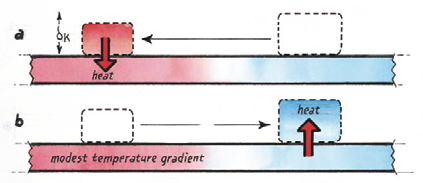
\includegraphics[width=0.8\textwidth]{images/powerofsound/gascycle.png}
  \caption{(a) gas shifted to one side gets compressed and warmed so that the gas releases heat to the solid (b) the same gas shifts to the right, expands and cools down and absorbs heats from the solid\cite{powerofsound}}\label{gascycle}
\end{figure}
\newpara{}
This cycle for a gas parcel plotted in a \(p-V\) diagram (Figure~\ref{pvstanding}) shows that there is work absorbed by the gas and is typical for a heat pump. The opposite is also true, a temperature gradient can be created along a solid by an external heat source. This temperature gradient causes the gas to compress and expand in the same way as discussed above but in reverse order. This device transforms heat into acoustic power and is consequently an engine. Such a device is called a \emph{thermoacoustic heat engine (TAHE)} or \emph{primer mover}. A diagram of these two different principles is shown in Figure~\ref{diagramengine}. TAHE are not the focus of this paper but will come up later because they are essential to some TAHP configurations.
\begin{figure}[ht]
  \centering
  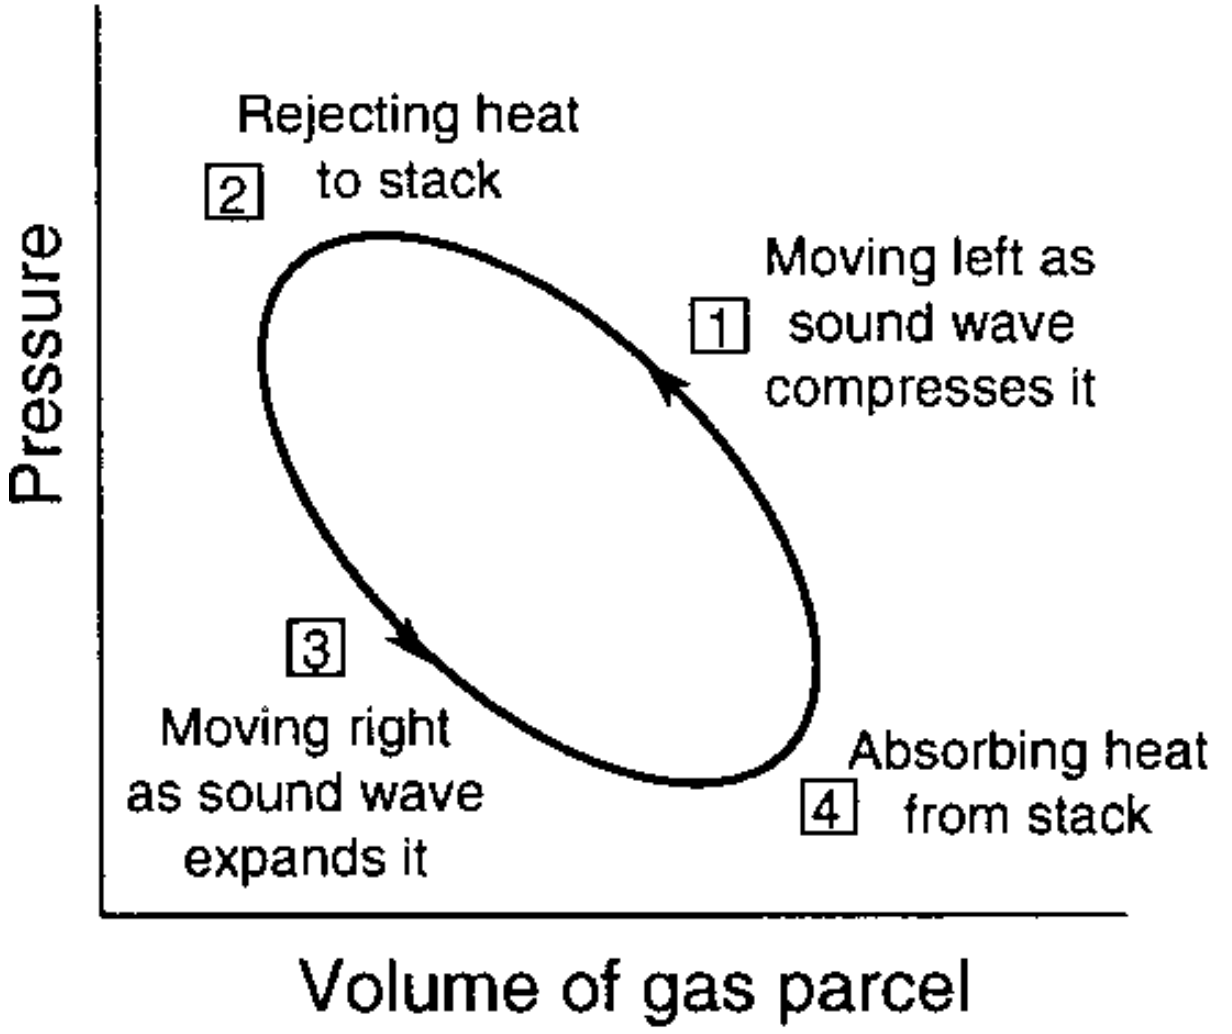
\includegraphics[width=0.8\textwidth]{images/pvstanding.png}
  \caption{\(p-V\) diagram showing the four stages of the thermoacoustic heat pumping process\cite{russell2002tabletop}}\label{pvstanding}
\end{figure}
\begin{figure}[ht]
  \centering
  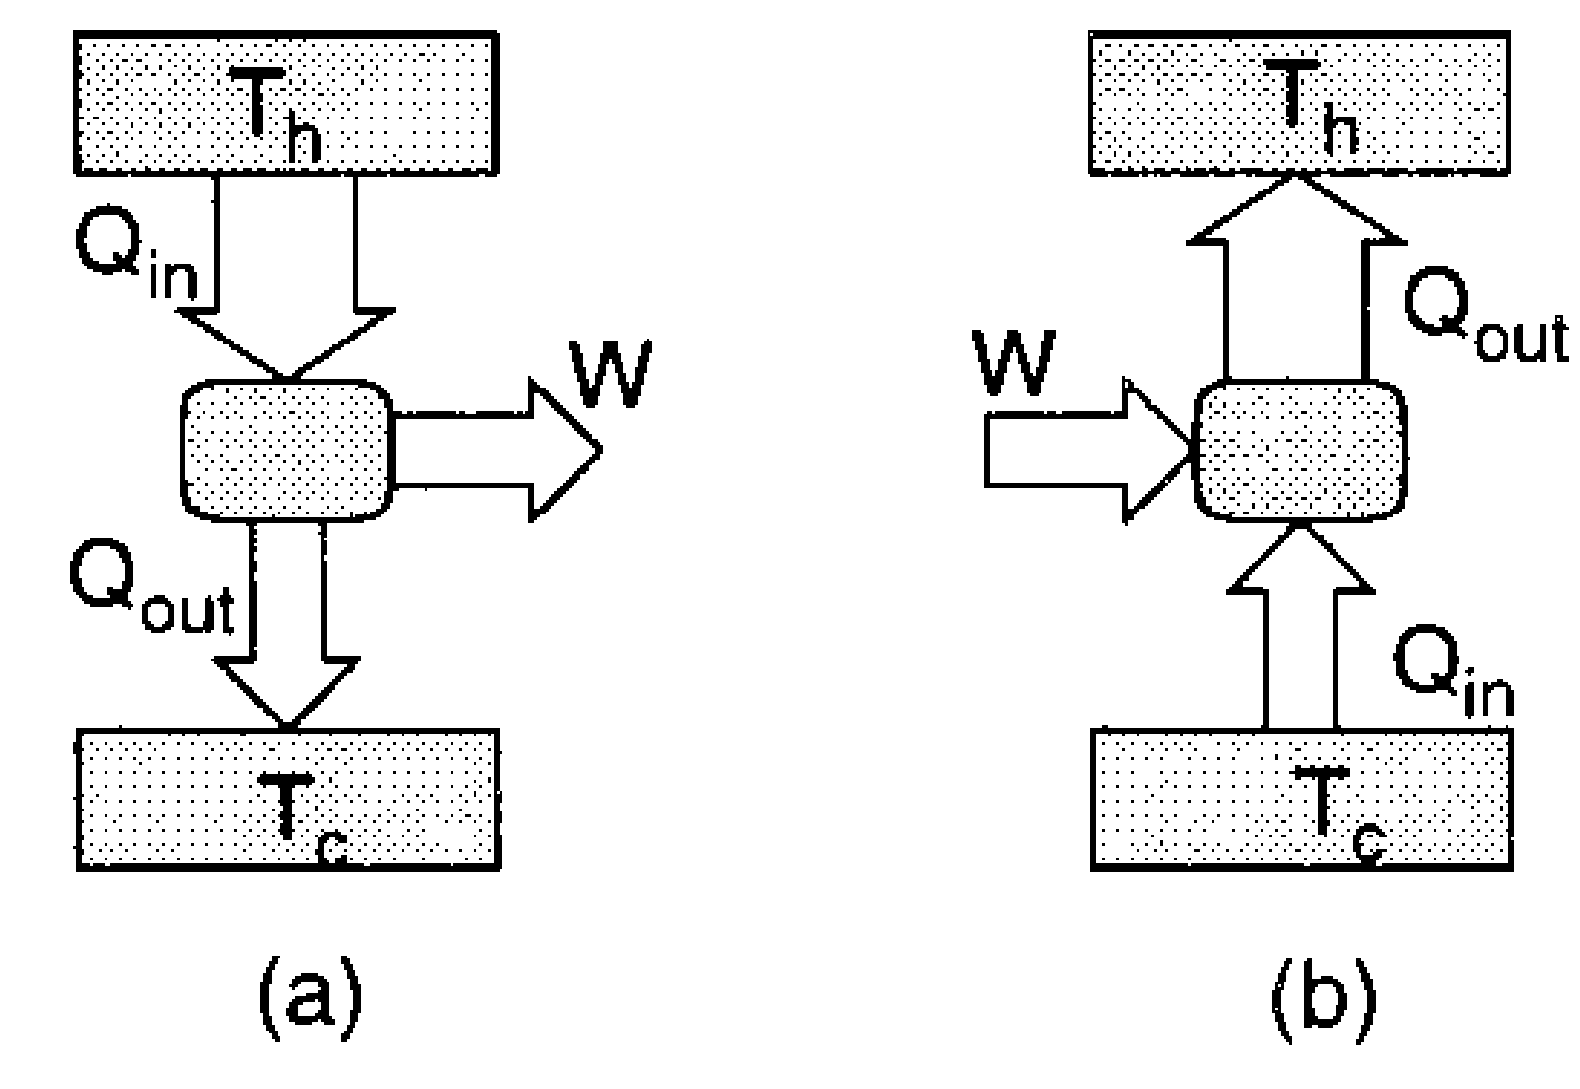
\includegraphics[width=0.5\textwidth]{images/diagramengine.png}
  \caption{(a) the working principle of TAHE where heat \(Q_{in}\) from an external heat source is transformed into acoustic power \(W\) (b) acoustic power \(W\) is transformed into useful heat flow~\(Q_{out}\) or \(Q_{in}\) depending on the TAHP being used for heating or refrigeration respectively\cite{russell2002tabletop}}\label{diagramengine}
\end{figure}
\newpara{}
The solid used in TAHP should have good thermal contact when the parcel is stationary but poor thermal contact when the parcel is moving. The solid should also not conduct heat from one end to the other and thus have a low thermal conductivity.  The quest of finding this material is a large part of making TAHP commercially viable, but plastic is often sufficient for experimental setups. This deliberate bad thermal contact makes standing wave TAHP inherently irreversible. This property is the major reason why the efficiency of these devices is limited. According to a study conducted by Zolpakar et al.\ the optimal material to date is mylar\cite{ZOLPAKAR2016626}.
\newpara{}
TAHP use a stack of plates of these solids to increase thermal efficiency. This stack is called the \emph{stack}. These plates are mounted parallel to each other with a specific distance between them. Detailed analysis shows that the optimal distance between these plates is about 3 times the \emph{thermal penetration depth}\cite{tijaniOptimalStack}. The thermal penetration depth is the distance over which thermal diffusion happens between the surface of a solid and a liquid.  % DISCUSS THIS FURTHER
\newpara{}
The most rudimentary form of a TAHP consists of a resonator, gas, stack, acoustic transducer, and hot and cold heat exchangers (Figure~\ref{tube}). The acoustic transducer applies acoustic power \(W\) to the gas in the resonator such that a standing wave of the first harmonic is formed in the resonator. A stack is located at about a fourth of the resonator length from the transducer and the resonator has a length of half the wavelength of the gas. A hot heat exchanger is mounted on the left at the side of the stack which is closest to a node where temperature and pressure will be at their maximum. A cold heat exchanger is then mounted on the right side closest to the anti-node where the temperature of the gas will be at its minimum.
\begin{figure}[ht]
  \centering
  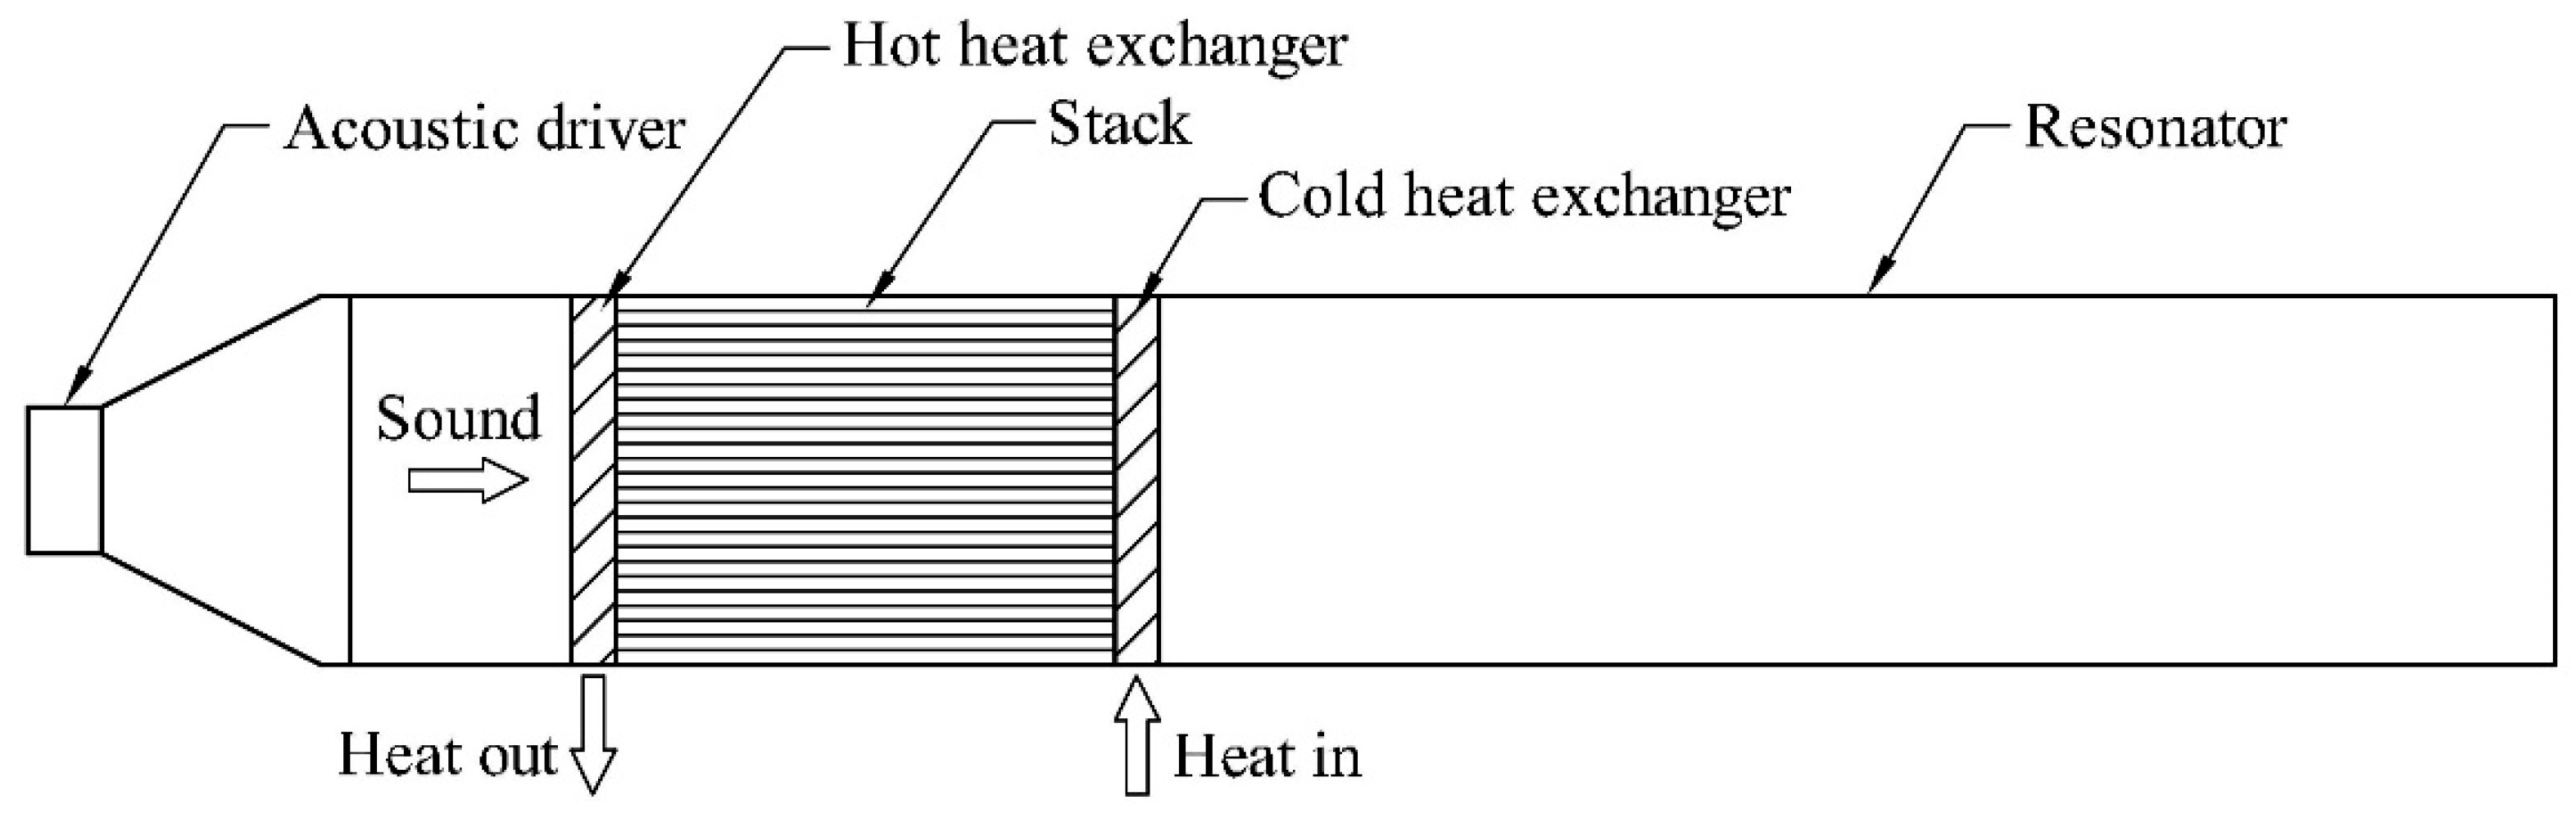
\includegraphics[width=0.8\textwidth]{images/tube.png}
  \caption{Simple standing wave thermoacoustic device\cite{en14010083}}\label{tube}
\end{figure}
\newpara{}
The choice of gas used in TAHP are often based on the thermoacoustic power density. Swift showed that this power density is proportional to the pressure and speed of sound of a gas\cite{book}. Noble gases, most notably helium, have high thermal conductivity and speed of sound and thus are often chosen. The high thermal conductivity increases the thermal penetration depth and thus the geometry of the stack. This allows for stacks to be manufactured without the need for precision engineering. The high speed of sound means that high-frequency devices can be constructed without the dimensions being too small.
\newpara{}
The bucket brigade of gas parcels pumps heat from the cold end of the stack to the hot end and creates a temperature gradient. In the case of a \emph{thermoacoustic refrigerator}, the cold heat exchanger is connected to a room to be cooled at \(T_c\), and the hot exchanger is connected to a heat sink at \(T_h\). This is reversed when the desired effect is the heating of a room. This technology is, however, the most promising in the former case.

\subsubsection{Efficiency and losses}
The efficiency for heat pumps, known as the \emph{coefficient of performance (COP)}, is limited by the second law of thermodynamics and is defined by the Carnot efficiency \(T_c/(T_h-T_c)\). The losses preventing this device from reaching Carnot efficiency are as follows:
\begin{description}
  \item[Inherent losses] Inherent losses are due to the irreversibility of the heat transfer between the stack and a gas parcel. Because the heat transfer happens across a non-zero temperature difference \(\delta T\), the entropy of the universe increases. This irreversibility is inherent to this device because of the imperfect thermal contact. % ADD FORMULA
  \item[Viscous losses] Viscous losses occur because the gas must overcome viscous shear forces in the stack. The \emph{viscous penetration depth} \(\delta_\mu=\sqrt{\mu / \pi f \rho} \) is comparable to the \emph{thermal penetration depth} \(\delta_\kappa\). Because the plates are spaced about four times this depth apart, the gasses undergo a significant amount of viscous shear.
  \item[Conduction losses] This loss occurs by the simple conduction of the hot end of the stack to the cold end of the stack.
  \item[Auxiliary losses] The losses discussed also happen in other parts of the device. Viscous and inherent losses also occur in other parts of the resonator, not necessarily in the stack, which also contributes to the losses. Conduction losses also occur through the casing of the resonator.
  \item[Transduction Losses] The acoustic transducer generating power for the system is also imperfect. In the case of an electrical system, i.e.\ a loudspeaker, the main losses will be Joule heating in the copper wires of the loudspeaker.
\end{description}
These losses combined cause simple standing-wave TAHP to be inefficient.
\newpara{}
Many optimizations have been studied by researchers throughout the years but the COPs of these systems are relatively low compared to conventional alternatives such as compression-based refrigeration. These parametric optimizations have been carried out either numerically or experimentally. The components subject to these optimizations are, among others, the stack, the resonator, the working fluid, etc.\ Zolpakar et al. tabulated the various findings by different researchers throughout the years and concluded the following:\cite{ZOLPAKAR2016626}:
\begin{enumerate}
  \item The stack geometry should optimize the thermal boundary layer such that gas parcels can move freely and such that the stack is manufacturable.
  \item The spacing between the stack plates should be around 3 thermal penetration depths.\cite{tijaniOptimalStack}
  \item Mylar is the optimal stack material to date because it has a low thermal conductivity and high heat capacity and is easily manufacturable.
  \item A mixture of noble gases offers the highest efficiency, but helium remains the best fluid for cooling power because of its high speed of sound which was discussed earlier.
  \item The frequency and pressure of the wave are also important. A higher frequency and pressure will lead to a higher power density but will decrease the thermal penetration depth exponentially. Most researchers opt for a frequency between 300 Hz and 500 Hz and pressure around the atmospheric pressure as a compromise between the two effects.
  \item Other types of resonators are also possible (Figure~\ref{resonators}). The gas inside a resonator tube can be viewed as three separate parts: the fluid that is inside the stack transferring heat, the fluid which is close to the wall of the resonator and is dissipating heat, and the rest which is compressing and expanding adiabatically. The quarter-wavelength tube from Figure~\ref{resonators}.b is used to minimize dissipative effects on the resonator. The buffer volume makes the resonator act as if it was open-ended whilst still keeping the system closed. Figure~\ref{resonators}.c improves the resonator by minimizing the surface of the resonator. Figure~\ref{resonators}.d improves further by minimizing the buffer volume and is considered to be the optimal resonator for standing wave TAHP.\@
\end{enumerate}
\begin{figure}[ht]
  \centering
  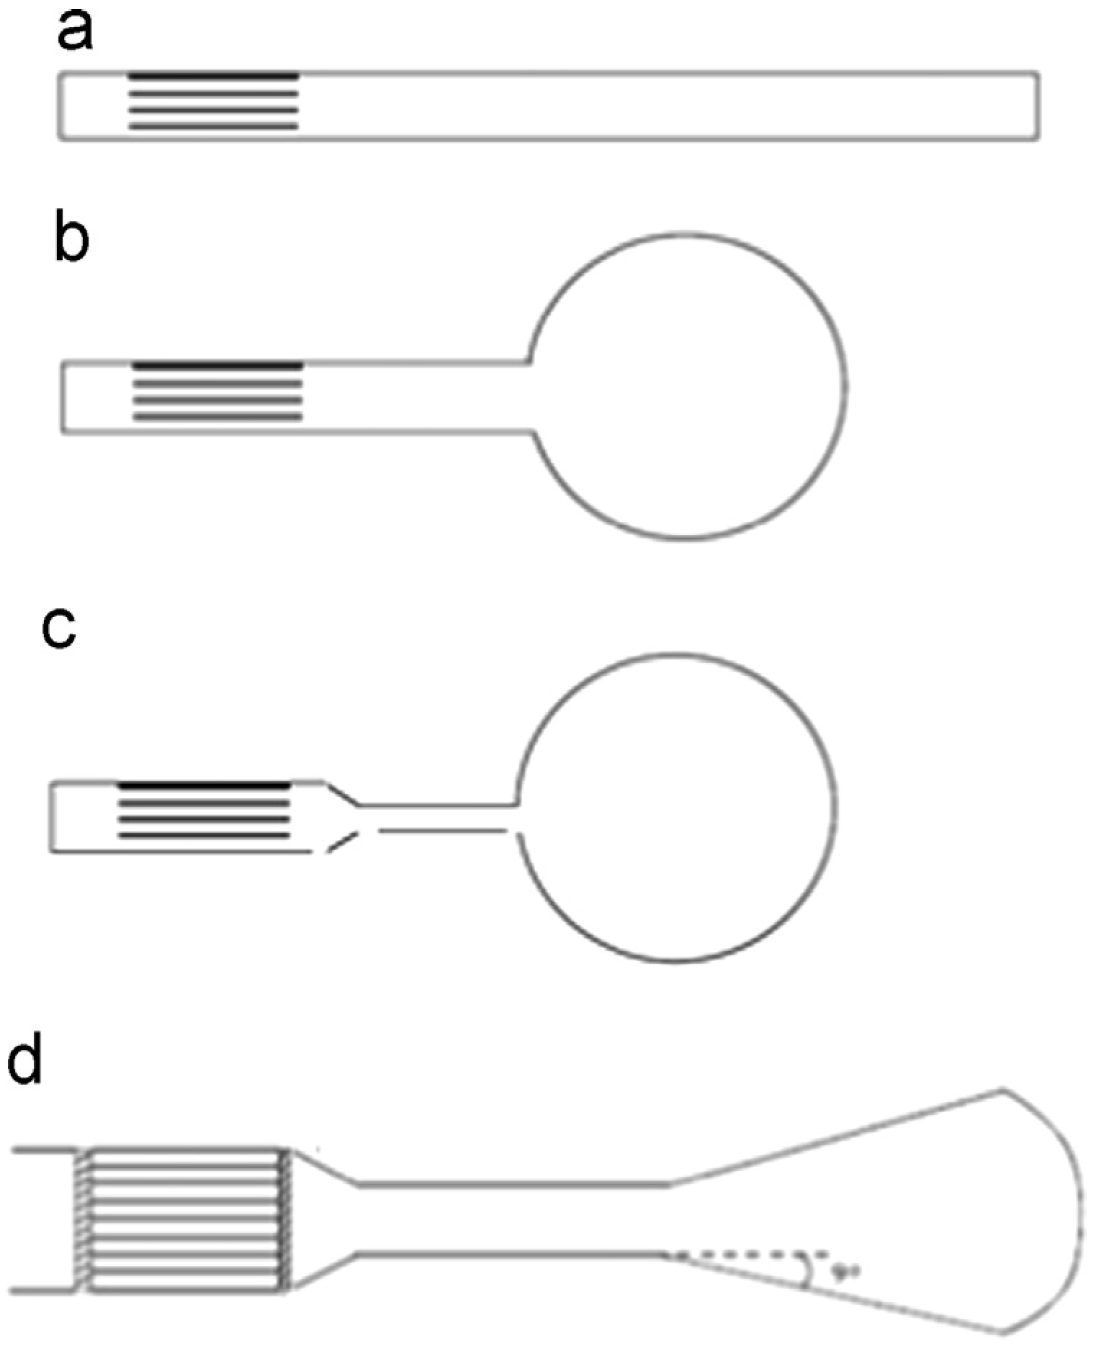
\includegraphics[width=0.5\textwidth]{images/resonators.png}
  \caption{Types of resonator: (a) half-wavelength (b) quarter-wavelength with sphere
    buffer volume (c) two-diameter resonator with sphere-buffer volume, and (d) two-diameter resonator with conical buffer volume.\cite{ZOLPAKAR2016626}}\label{resonators}
\end{figure}

The highest theoretical COP achieved by these optimizations is a COP of 3 by Minner et al.\cite{minner1996optimizing} which is still not sufficient and will probably be even lower for a real-world application.
\newpara{}
Standing wave TAHP should, however, not be immediately discarded. The efficiency of these devices can still be improved. Furthermore, almost no moving parts are required. In the case where a loudspeaker is used only a simple seal like a metal bellow would suffice and there would be no need for lubrication. There is also the possibility of coupling the TAHP with a thermoacoustic heat engine which means that there would be no moving parts at all. In this configuration, waste heat from e.g. an industrial installation would power a thermoacoustic heat engine producing acoustic power which would then be fed to a TAHP to cool down or heat a space for example.
\newpara{}\
The efficiency of standing wave systems is imposed by the way that heat is transferred from the stack to the gas which is similar to the Brayton cycle and is inherently irreversibly due to the bad thermal contact. Researchers have found a way to use a different thermodynamic cycle, the Stirling cycle, to improve the efficiency of thermoacoustic devices.\cite{ceperleyStirling}

\subsection{Traveling Waves\cite{spoelstraHighTemperature,BackHauseDetailedStudy,powerofsound,weiTravellingwave}}
In contrast to the inherently irreversible thermodynamic cycle which standing wave TAHP use, the reversed Stirling cycle is inherently reversible because it allows for optimal thermal contact. By finding a TAHP which uses this reverse Stirling cycle it is possible to surpass the efficiency of standing wave TAHP.\@

\subsubsection{Stirling cycle}
The Stirling cycle for a Stirling engine with a regenerator consists of four different steps which are plotted in a \(p-V\) diagram in Figure~\ref{stirlingcycle}:
\begin{enumerate}[(a)]
  \item Isothermal heat removal (compression)
  \item Isochoric heat addition (constant volume)
  \item Isothermal heat addition (expansion)
  \item Isochoric heat removal (constant volume)
\end{enumerate}
\begin{figure}[ht]
  \centering
  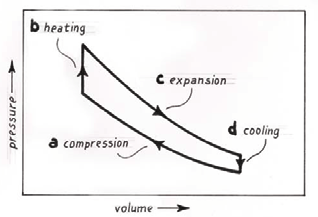
\includegraphics[width=0.5\textwidth]{images/powerofsound/stirlingcycle.png}
  \caption{The Stirling cycle\cite{powerofsound}}\label{stirlingcycle}
\end{figure}
The gas velocity and pressure for the gas in a sterling engine's regenerator are plotted alongside the gas velocity and pressure of a traveling wave in Figure~\ref{pvstirling}. This Figure clearly shows that a traveling wave undergoes a stirring cycle because the gas velocity and pressure are in phase (this is not the case in standing waves). The regenerator is a porous material, not unlike a stack, that stores thermal energy in part of the cycle and returns it later.
\begin{figure}[ht]
  \centering
  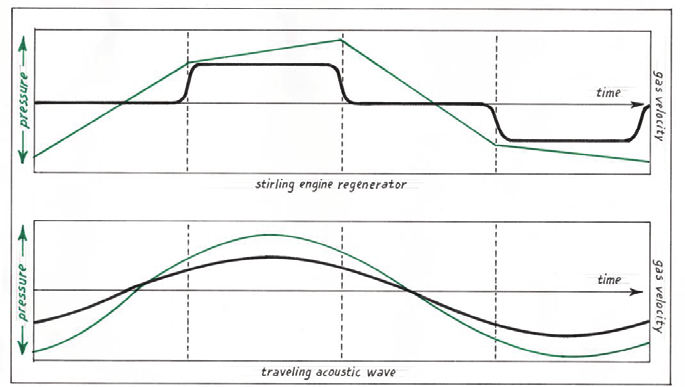
\includegraphics[width=0.8\textwidth]{images/powerofsound/pvstirling.png}
  \caption{The changes in pressure and gas velocity within the regenerator of a Stirling engine mimic the relationship
    seen in a traveling acoustic wave, where pressure and gas velocity move up and down in phase\cite{powerofsound}}\label{pvstirling}
\end{figure}
\newpara{}
Ceperley\cite{ceperleyStirling} showed that a TAHE could be created by creating a temperature gradient across a regenerator and sending a traveling wave through it. Thermal energy from the regenerator was converted into acoustic power. A schematic of the device that Ceperley built is shown in Figure~\ref{ceperley}. Ceperley was not successful in building a device that could do this efficiently, but through years of research and experimentation by his peers, TAHE using traveling waves became the most efficient and promising form of TAHE.\@ As with standing wave TAHE, when the cycle is reversed a TAHP is created, meaning that when a traveling wave with sufficient acoustic energy is forced through a regenerator it is possible to cool or heat.
\begin{figure}[ht]
  \centering
  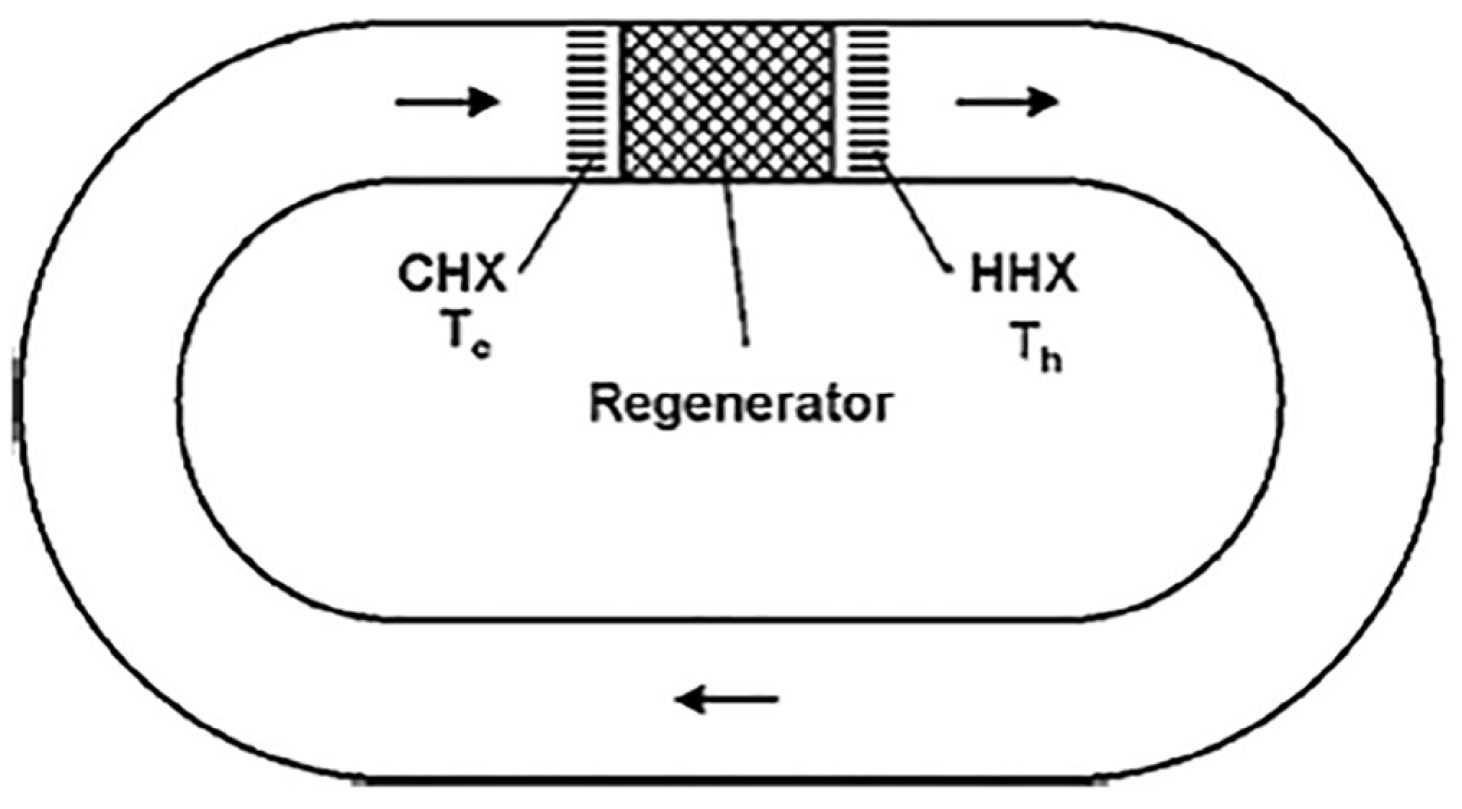
\includegraphics[width=0.8\textwidth]{images/ceperley.png}
  \caption{Schematic of a simple traveling wave thermo-acoustic system\cite{powerofsound}}\label{ceperley}
\end{figure}

One of the main differences between a traveling wave and a standing wave TAHP is the regenerator. The regenerator is a porous solid with a high heat capacity. These pores are smaller than the thermal penetration depth and thus much smaller than the gaps in a stack. These smaller pores, however, ensure better thermal contact and makes it possible for the device to be reversible in theory.
\newpara{}
The losses in the regenerator are proportional to the square of the oscillating velocity of the gas. This is analogous to the power dissipated in an electrical resistor which is proportional to the square of the current. Electrical engineers solved this similar problem for transmission lines by lowering the current and increasing the voltage. Garrett and Backhaus\cite{powerofsound} reasoned that the way electrical engineers solved this problem could also apply to the acoustically analogous case. This means that the velocity of the gas should be minimized and the oscillatory pressure should be maximized to increase efficiency. A traveling wave TAHP should thus have a wave that has the oscillatory pressure and velocity in phase whilst also minimizing the oscillatory velocity in the regenerator. Standing waves have a high pressure-to-displacement ratio, a traveling wave TAHP should thus incorporate the best of both worlds to maximize efficiency.
\newpara{}
A widely adopted design for traveling wave TAHP combines a standing wave resonator and a torus-like device containing the regenerator (See figure X). The torus is comprised of a hot heat exchanger (HHX), a regenerator (REG), a cold heat exchanger (CHX), a thermal buffer tube (TBT), an ambient heat exchanger (AHX), and a feedback inertance. The standing wave in the resonator moving along the open end of the torus acts like air blowing over the mouth of a bottle. The springiness of the gas in the inertance tube allows a wave of high pressure and low displacement (standing wave property) with the velocity and pressure in phase (traveling wave) to develop. The combination of these properties makes this specific configuration one of the most efficient methods of thermoacoustic refrigeration. The acoustic network formed by these elements forces a traveling wave to travel anti-clockwise in the torus and make the gas perform a reverse Stirling cycle in the regenerator and thus pumping heat away from the CHX.\@ The TBT and AHX are there to prevent heat from leaking.\cite{TijaniAHighPerformanceThermoacousticEngine}.
\newpara{}
One major problem with this design is that it does not inhibit Gedeon streaming i.e.\ air circulating from one end of the loop to the other and thus short-circuiting the CHX and HHX.\@ This phenomenon drastically impacts efficiency and should be avoided. A flexible membrane installed just above the HHX would inhibit the flow of gas whilst still transmitting the acoustic power but can be difficult to develop in such a way that it lasts a long time. Another way is to use a jet pump. A jet pump creates a backpressure in the loop to inhibit the streaming by using asymmetric openings that allow flow in one direction.

\subsubsection{Efficiency}
Various designs have been tested numerically or experimentally since Ceperly first wrote his paper in 1979. The most promising are the looped-based designs as discussed above but efficiencies are still poor and insufficient for commercial viability. There are also different aims of these devices. Some traveling wave TAHP have been designed to liquefy hydrogen where cooling power is important while some designs focus more on room temperature applications where efficiency and power density are important\cite{WangRoomTemperature}.
\newpara{}
Tijani et al.\cite{spoelstraHighTemperature} built a traveling wave TAHP by building on the design discussed above. They coupled the TAHP with a TAE using the same principle but with a reversed cycle. This makes this device thermally driven. They managed to get to 40\% of Carnot's performance working between a range of 80 degrees and 10 degrees Celcius and pumping 200 W. This was an encouraging result for further study in this domain.
\newpara{}
Luo et al.\ built a refrigerator using the design discussed above\cite{LuoRefrigerator}. They also did this by coupling a traveling wave TAHP with a TAE in the same system but in a different way than the previous example. This device only reached a COP of 0.216 but managed to pump 469 W.
\newpara{}
More recently, Wang et al.\ estimated numerically that a refrigerator could be built with a cooling power of 6.35 kW and a COP of 3. This was built on the principle of putting multiple regenerators in series and thus creating a multistage refrigerator. Real-world experimentation is required however to validate these results.
\newpara{}
An in-depth study on the efficiency of traveling wave TAHP by Ueda et al.\ showed that three parameters mainly affect the efficiency of the regenerator: the regenerator's installation position, length, and flow-channel radius\cite{uedaOptimization}. They concluded that by optimizing these three parameters a COP of above 60\% of the Carnot COP could be achieved. Tartibu investigated the effect of different geometries and thus configurations of traveling wave TAHP and tabulated different findings of different researchers\cite{TARTIBU2019102}. His study shows that whilst traveling wave TAHP are not sufficiently efficient yet, they show great promise and have much higher potential than their standing wave counterparts.

\section{Applications}
This section will discuss real-world applications of TAHP.\@ There are not a lot of real-world applications outside of academia because of the infancy of this technology.
\subsection{Space applications}
Thermoacoustic applications are a good fit for space missions because of their reliability and energy density. In this section, I list two important applications.
\subsubsection{Space shuttle get-away-special (GAS)\cite{AdeffSpace,powerofsound}}
Two standing-wave TAHP were designed, tested, and certified by NASA for its launch of the GAS space shuttle in 1992. One component was devised to cool the urine and blood samples of astronauts the other component was designed to cool electronic components.
This TAHP was built by putting two standing wave TAHP in a stereo configuration as seen in Figure \ref{stereoStandingWave} and used a mixture of helium and xenon as the working fluid. The device only achieved 17\% of the Carnot efficiency. The refrigerator itself, however, achieved 26\% of the maximum which is only half of what conventional cooling systems of similar shape can achieve which was impressive for the novelty of the technology.
\newpara{}
Due to an abrupt stop of funding the project was never realized. Because the technology was promising, it was later picked up by the US Navy to cool radar electronics.
\begin{figure}[h]
  \centering
  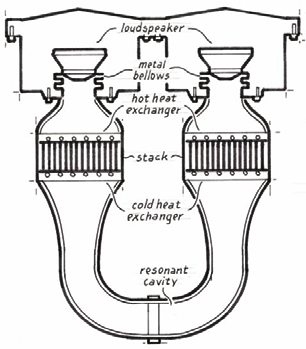
\includegraphics[width=0.5\textwidth]{images/powerofsound/stereo.png}
  \caption{Inner workings of the thermoacoustic refrigerator used to cool radar electronics: A pair of loudspeakers drives gas through two porous stacks attached to heat exchangers through which water circulates.\cite{powerofsound}}\label{stereoStandingWave}
\end{figure}

\subsubsection{JWT cryocooler\cite{Petach2014MidII,Moore_2017,ross2022conceptual}}
The James-Webb telescope (JWT) is a space telescope launched by NASA on 25 December 2021. The purpose of JWT was to conduct infrared astrology. Due to redshift, the light coming from very old and distant celestial bodies have a wavelength in the infrared range. The temperature of the mid-infrared camera (MIRI) aboard the JWT has to be as close to 0 kelvin as possible to minimize the infrared radiation of the telescope itself and thus minimize the noise.
\newpara{}
The heat shield of the JWT only manages to keep the temperature of the sensor at about 37 kelvin but the sensor has an operating temperature of 6.2 kelvin. NASA chose a thermoacoustic cooler because reliability, high cooling power, and energy density were key. The cryocooler is a standing wave TAHP operating on helium with three stacks. A tube of helium is connected to the cold heat exchangers of the TAHP and is cooled down to about 17 kelvin which is still not enough which is still not sufficient. At the end of the tube, there is a small hole that drops the pressure of the helium. Because of this Joule-Thompson effect, the helium cools down to 6.2 kelvin to finally cool the MIRI.\@ So far, this cooler has worked successfully and is expected to for the coming 18 years.

\subsection{Domestic applications}
Almost 80\% of domestic heating in Europe is still being done with fossil fuels according to the EU\cite{EU}. There are two startups in Europe seeking to improve these numbers by making heat pumps a more accessible and environment-friendly option.
\subsubsection{Blue Heart\cite{blueheart}}
Blue Heart is a Dutch spinoff of the Organisation for Applied Scientific Research (TNO) (Figure~\ref{blueheart}). A Blue Heart device would replace the cold circuit of a heat pump. The high energy density of TAHP reduces the space needed for heat pump installations. They developed a traveling wave TAHP with helium as the working fluid. The acoustic power is generated by two pistons opposite to each other moving at the same frequency. The vibrations get canceled making the TAHP more silent than their conventional compression-based counterparts. Blue Heart claims that its device works efficiently with every temperature input and output and has a larger operation envelope than compression-based heat pumps. They also claim to be compatible with every type of heat source and to be suitable for new and existing houses.
\newpara{}
A Blue Heart device would operate with source temperatures between -20 degrees to 50 degrees Celsius and with sink temperatures between 7 degrees and 80 degrees Celsius. It would also have a capacity of 6 kW. The company plans to make the device commercially available in 2024.
\subsubsection{Equium\cite{equium}}
Equium is a French startup that offers to replace the heat pump entirely in contrast to Blue Heart (Figure~\ref{equium}). The company has not revealed the inner workings of their device but it is expected to also be a traveling wave TAHP working with helium. The company promises an impressive maintenance-free lifetime of 30 years. These devices are also planned to be commercially available in 2024
\begin{figure}[h]
  \centering
  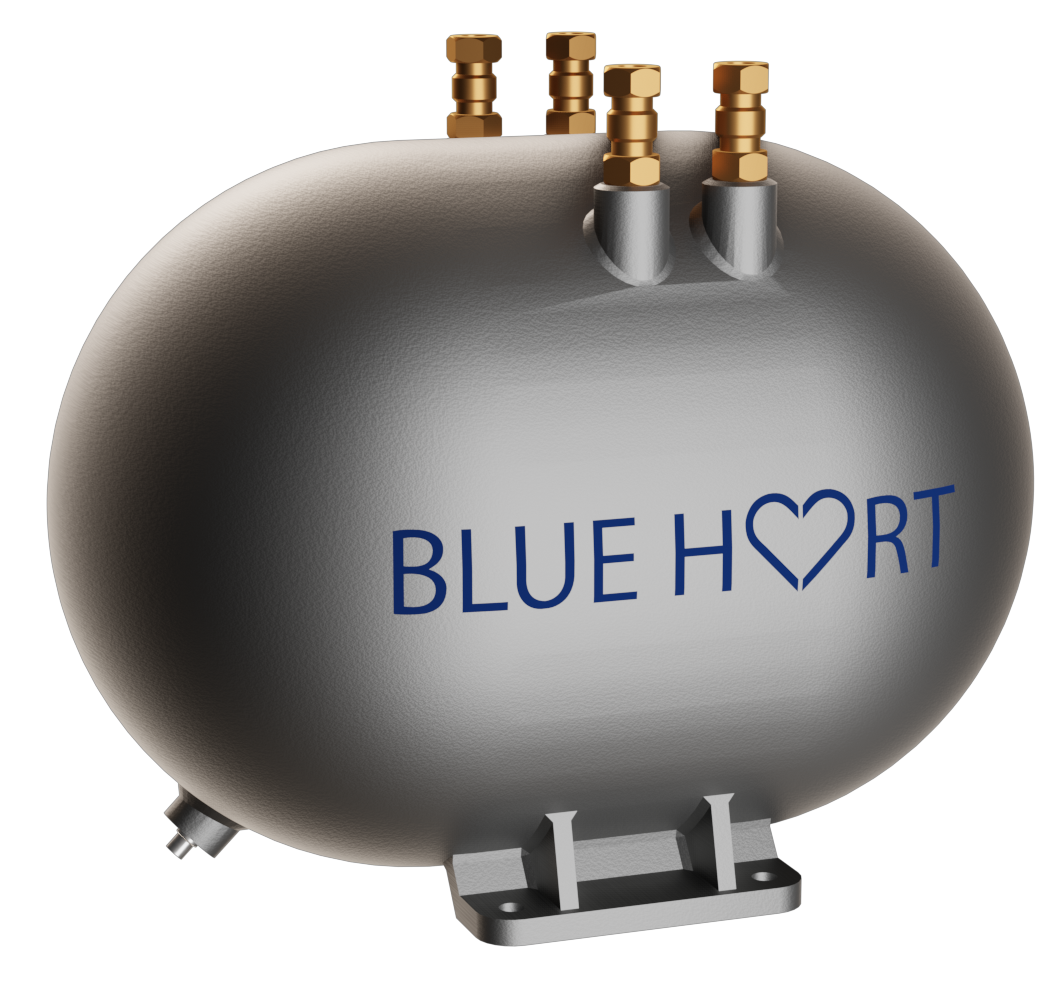
\includegraphics[width=0.5\textwidth]{images/blueheart.png}
  \caption{Blue Heart thermoacoustic device\cite{blueheart}}\label{blueheart}
\end{figure}
\begin{figure}[h]
  \centering
  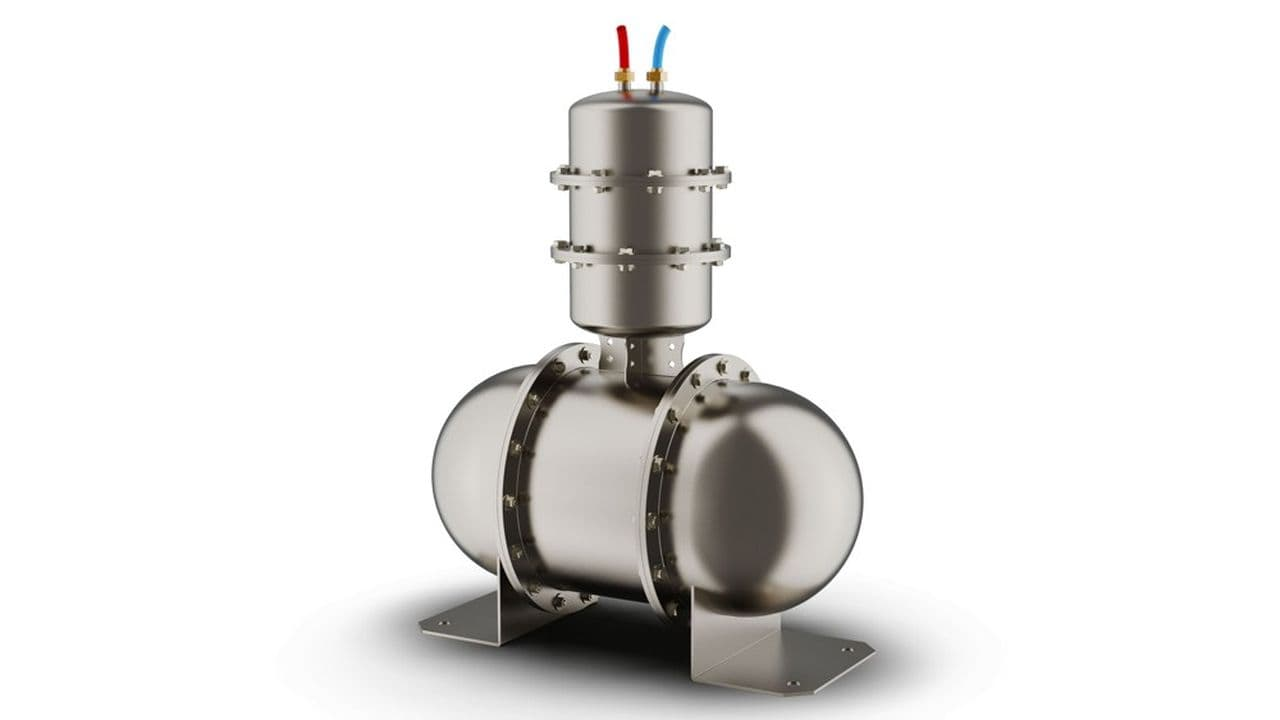
\includegraphics[width=0.5\textwidth]{images/equium.jpg}
  \caption{Equium Heart thermoacoustic device\cite{equium}}\label{equium}
\end{figure}
\subsection{Automotive applications}
Current refrigeration and cooling systems in automotive applications, based on compression, draw a lot of power from the engine and degrades the overall efficiency of the vehicle. Furthermore, the refrigerant often leaks from the system and is made of ozone-depleting material. An environment-friendly and efficient alternative to cooling systems in vehicles is thus crucial.
\newpara{}
Zoontjens et al.\ did a feasibility study on TAHP in automotive applications\cite{zoontjens2005feasibility}. They specifically studied the possibility of a thermally driven TAHP driven by recovered waste heat from waste exhaust gasses. They also compared this alternative to other prominent alternatives such as active magnetic resonator systems, solid adsorption cooling systems, vapor absorption refrigeration systems, etc.  What makes TAHP appealing, in this case, is the possibility to be driven thermally because combustion engines have low thermal efficiencies and thus release a significant amount of heat to the environment. A diagram of the system they devised is shown in Figure~\ref{automotiveDiagram} (ATAR stands for automotive thermoacoustic refrigeration).
\begin{figure}[h]
  \centering
  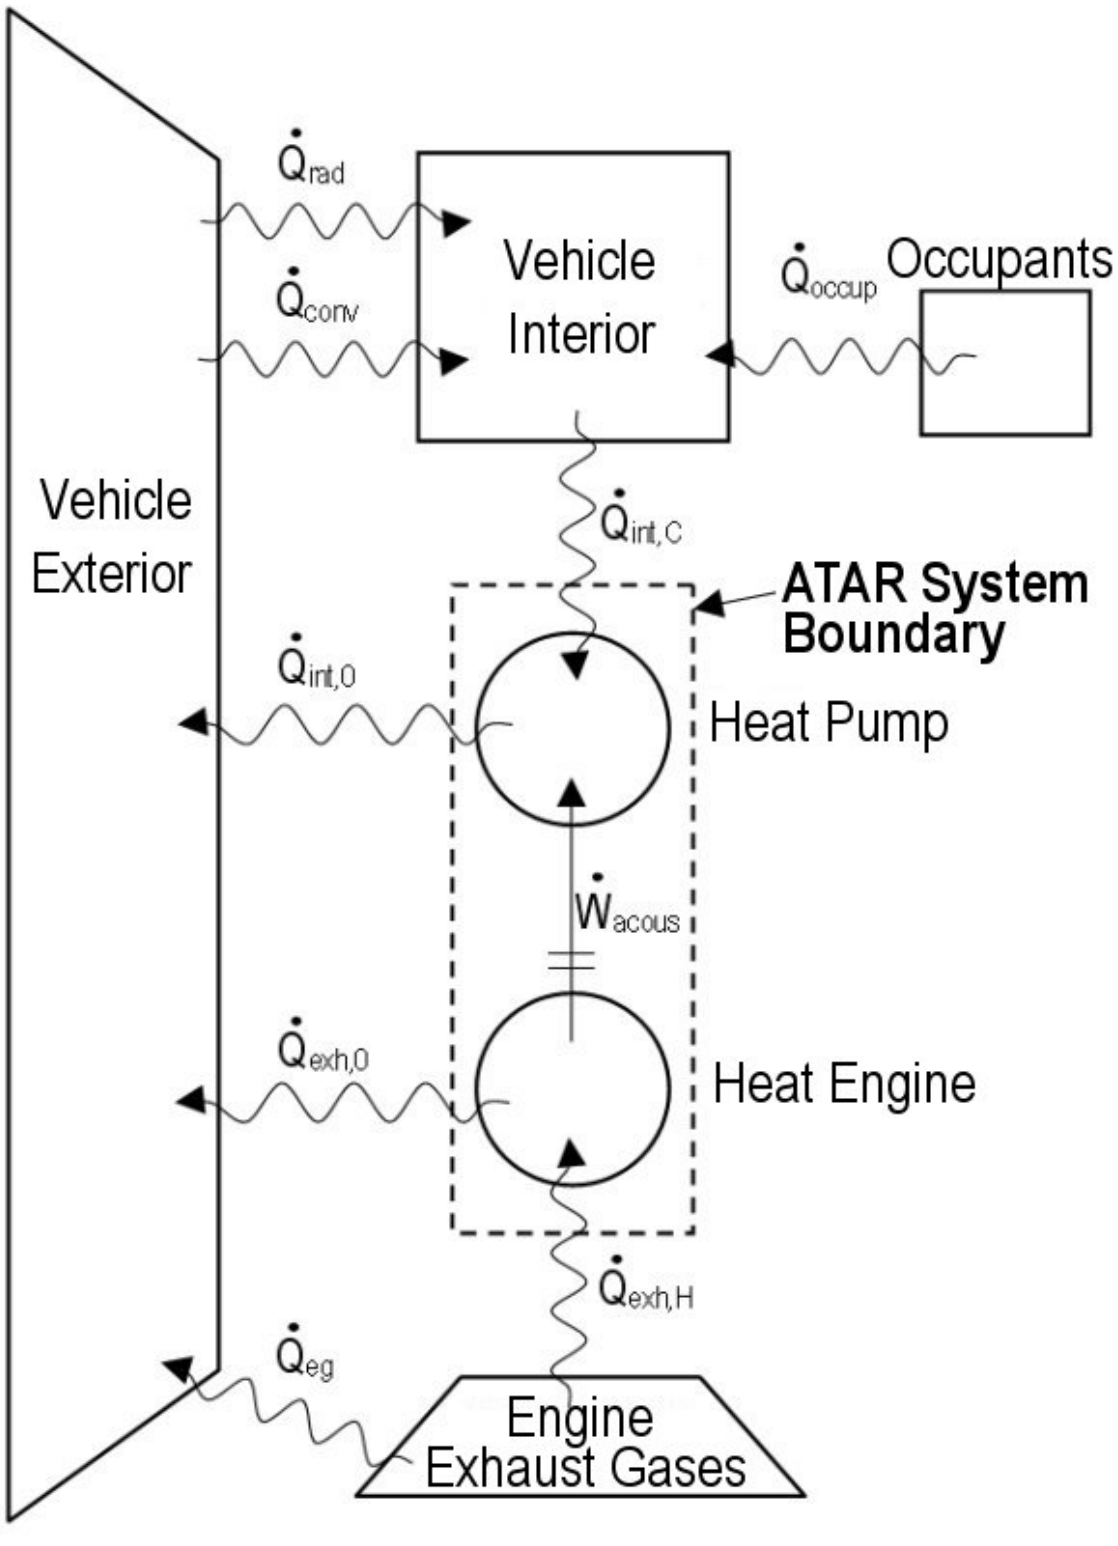
\includegraphics[width=0.5\textwidth]{images/automotive.png}
  \caption{Diagram of automotive thermoacoustic refrigerator\cite{zoontjens2005feasibility}}\label{automotiveDiagram}
\end{figure}
The implementation chosen for this study was a standard quarter-wavelength standing wave TAHP as discussed above. The two major concerns are cooling power and available heating power. The cost of developing a production-ready system of this kind is a big challenge to overcome. Especially with the ever-decreasing demand for combustion engine vehicles. The researchers found that these systems would be feasible but that further optimization and research will be necessary.
\section{Future challenges and limitations}

\section{Conclusion}
While efficiencies are not yet at the same levels as conventional cooling/heating applications, one should keep in mind that TAHP offers other important advantages. For example, they use inert gases which make them environment friendly. They are also very flexible in driver methods. They can be powered thermally and mechanically. They also have nearly no moving parts which makes them very suitable for environments where reliability is key.
\newpage
\bibliography{uni}
\bibliographystyle{unsrt}
\end{document}
